\documentclass[a4paper, oneside, 11pt, onecolumn]{article}
\usepackage[T1]{fontenc}
\usepackage{newtxtext,newtxmath}
\usepackage{graphicx}
\usepackage{subfigure}
\usepackage[round, comma, sort&compress, longnamesfirst]{natbib} 
% \usepackage[left=2cm,top=3cm,right=1.5cm,bottom=2cm,bindingoffset=0.5cm]{geometry}
\usepackage{enumerate}
\usepackage{fancyhdr}
\usepackage[title,titletoc,toc]{appendix}
\pagestyle{fancy}
\fancyhead{}
\fancyfoot{}
\fancyfoot[L]{\textit{running footer}}
 \fancyhead[L]{\textit{running title}}
\renewcommand{\headrulewidth}{0.8pt}
\renewcommand{\footrulewidth}{0.8pt}
\setlength\headheight{14pt}
\fancyfoot[RO] {\thepage}
\usepackage{authblk}
%%%%%%%%%%%%

\begin{document}

\title{Individual Differences Across Visual Search Tasks}

\author{A. D. F. Clarke, J. L. Irons, A. B. Leber and A. R. Hunt}
\affil{Aberdeen, Essex and Ohio}

\maketitle

\begin{abstract}
Some abstract goes here
\end{abstract}

%%%%%%%%%%%%%%%%%%%%%%%%%%%%
\section{Introduction}
%%%%%%%%%%%%%%%%%%%%%%%%%%%%


%%%%%%%%%%%%%%%%%%%%%%%%%%%%
\section{Methods}
%%%%%%%%%%%%%%%%%%%%%%%%%%%%


\subsection{Participants}
How many? Will all testing be done at the University of Aberdeen? How do we justify our sample size (a question commonly asked by journals now!)?

\subsection{Materials and Procedures}

The study consists of three different paradigms from the visual search literature in which strong individual differences were found \citep{nowakowsak2017, irons-leber2016, kristjansson2014}.
{}
\subsubsection{A: Split-half array search}

\subsubsection{B: Attentional Control}

\subsubsection{C: Conjunction Foraging}

\subsection{Planned Analysis}

\subsubsection{A: Split-half array search}

In order to characterise an individual's behaviour in this task, we will compute the proportion of the first $n$ fixations that were on heterogeneous (difficult) side of the stimuli, over all target absent trials\footnote{Only take correct trials?}. \cite{nowakowsak2017} demonstrated a strong correlation between an this metric (for $n=5$) and reaction times ($r=$). However, a re-analysis of their data shows that an even stronger correlation is obtained with $n=3$ (see Figure \ref{fig:nowakowskaBestN})

\begin{figure}
\centering
\subfigure[][]{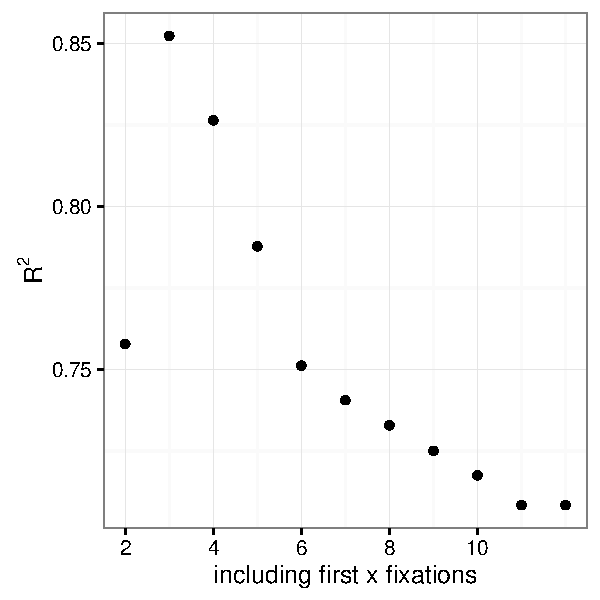
\includegraphics[width=6cm]{../NowakowskaClarkeHunt2017/scripts/r_by_nfix.pdf}}
\subfigure[][]{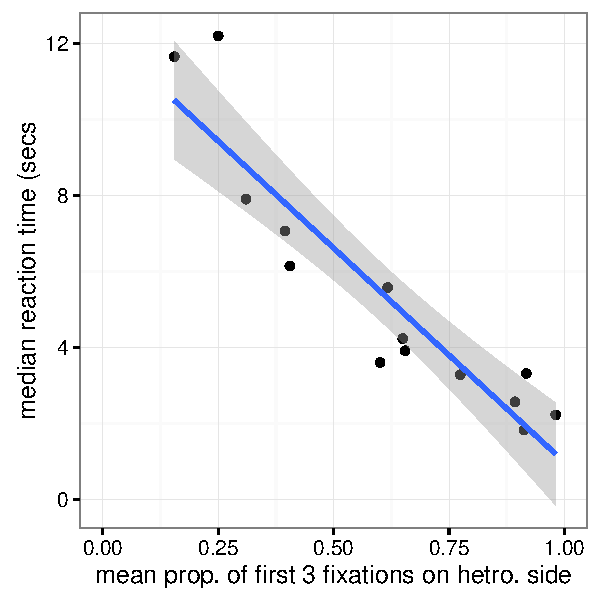
\includegraphics[width=6cm]{../NowakowskaClarkeHunt2017/scripts/best_r_scatter.pdf}}
\caption{Selecting the best $n$.}
\label{fig:nowakowskaBestN}
\end{figure}

\subsubsection{B: Attentional Control}

\subsubsection{C: Conjunction Foraging}

\subsubsection{}


\subsection{Exploratory Analysis}

We will carry out additional analysis, above and beyond what has been documented above, but the exact nature of this will be contingent on the nature of the results. Something like PCA may be interesting. 

%%%%%%%%%%%%%%%%%%%%%%%%%%%%
\section{Results}
%%%%%%%%%%%%%%%%%%%%%%%%%%%%

%%%%%%%%%%%%%%%%%%%%%%%%%%%%
\section{Discussion}
%%%%%%%%%%%%%%%%%%%%%%%%%%%%


%%%%%%%%%%%%%%%%%%%%%%%%%%%%
\begin{appendices}
\section{Hetero-Homo-geneous Array Search}
%%%%%%%%%%%%%%%%%%%%%%%%%%%%

%%%%%%%%%%%%%%%%%%%%%%%%%%%%
\section{Attentional Control Settings}
%%%%%%%%%%%%%%%%%%%%%%%%%%%%

%%%%%%%%%%%%%%%%%%%%%%%%%%%%
\section{Conjunction Foraging}
%%%%%%%%%%%%%%%%%%%%%%%%%%%%
\end{appendices}

\bibliographystyle{plainnat}
\bibliography{literature}

\end{document}


